\documentclass[12pt,a4paper]{report}

\usepackage[utf8]{inputenc}
\usepackage{graphicx}
\usepackage{geometry}
\usepackage{setspace}
\usepackage{subcaption}
\usepackage{amsmath}
\usepackage{algorithm}
\usepackage{algorithmic}
\usepackage{tabularx}
\usepackage{float}
\usepackage{comment}

\geometry{
  a4paper,
  top=35mm,
  bottom=30mm,
  left=40mm,
  right=25mm
}

\usepackage{titlesec}

\titleformat{\chapter}[display]
  {\normalfont\bfseries\centering}
  {CHAPTER \thechapter}
  {1\baselineskip}
  {\Large}

\titlespacing*{\chapter}
  {0pt}
  {15mm}
  {1\baselineskip}



\onehalfspacing


\begin{document}

\pagenumbering{roman}

%--------Title page -----------


\begin{titlepage}
\begin{center}
{\fontsize{18}{22}\selectfont
\textbf{Quantum CryptAnalysis of Block Cipher \\ using Grover’s Algorithm}
}


\vspace{12mm}

A REPORT ON PROJECT WORK (PHASE II)

\vspace{8mm}

Submitted in partial fulfillment of the requirements for the award of the degree of

\vspace{8mm}

\textbf{MASTER OF TECHNOLOGY}

\vspace{4mm}

in

\vspace{4mm}

\textbf{COMPUTER SCIENCE AND ENGINEERING}

\vspace{12mm}

by

\vspace{4mm}

\textbf{Vidit Odedra}\\
(Roll No: 206124035)

\vspace{5mm}


\includegraphics[width=0.3\textwidth]{NITT_logo.png}

\vspace{12mm}

\textbf{DEPARTMENT OF COMPUTER SCIENCE AND ENGINEERING}\\
\textbf{NATIONAL INSTITUTE OF TECHNOLOGY}\\
\textbf{TIRUCHIRAPPALLI – 620015}

\vspace{8mm}

\textbf{January 2026}

\end{center}
\end{titlepage}


%---------------- Certificate --------------

\cleardoublepage
\setcounter{page}{2}
\doublespacing

\begin{center}
\textbf{BONAFIDE CERTIFICATE}
\end{center}

\vspace{2\baselineskip}

This is to certify that the thesis entitled \textbf{“Quantum CryptAnalysis of Block Cipher using Grover’s Algorithm
”} is a bonafide record of the work done by \textbf{Vidit Odedra}, studying in Master of Technology (Computer Science and Engineering) in the National Institute of Technology, Tiruchirappalli, during the academic year 2025–2026.

\vspace{30mm}

\noindent
\textbf{Dr. Kunwar Singh} \hfill \textbf{Dr. Kunwar Singh}\\
Guide \hfill Head of the Department\\
Department of Computer Science and Engineering\\
National Institute of Technology, Tiruchirappalli

\vspace{20mm}

\noindent
Project Viva-Voce held on: \rule{5cm}{0.4pt}

\vspace{10mm}

\noindent
Internal Examiner \hfill External Examiner

%---------- Abstract ----------------------------
\cleardoublepage
\setcounter{page}{3}
\onehalfspacing

\begin{center}
\textbf{ABSTRACT}
\end{center}

Quantum computing introduces new threats to symmetric cryptography by enabling faster exhaustive key search through algorithms such as \textbf{Grover's algorithm}. Although symmetric block ciphers remain resistant to many classical attacks, Grover's algorithm reduces their effective security by providing a \textbf{quadratic speedup} in key search. Therefore, estimating the quantum resources required to attack practical symmetric ciphers is an important problem in the context of \textbf{post-quantum cryptography}.

In this thesis, a \textbf{reversible quantum circuit implementation of the PRINCE block cipher} is presented and analyzed. PRINCE is a lightweight symmetric block cipher with a \textbf{64-bit block size} and a \textbf{128-bit key}, designed for low-latency hardware applications. The proposed quantum implementation reproduces the classical encryption structure of PRINCE using reversible quantum operations, including S-box layers, linear M-layers, round-key additions, round constants, and the PRINCE key schedule. Since the circuit is reversible, it can be embedded within a \textbf{quantum oracle}, which is required for applying Grover's algorithm to key search.

To study a Grover-based attack, the PRINCE encryption circuit is used inside an oracle that checks whether a candidate key maps a known plaintext to a target ciphertext. The key register is placed in a \textbf{superposition of all possible 128-bit keys}, and one Grover iteration is constructed using the encryption oracle, phase marking, uncomputation, and the Grover diffuser. However, simulating the full quantum state of a 128-bit key search would require tracking an infeasible number of amplitudes, namely \textbf{$2^{128}$} key states. Therefore, this work focuses on \textbf{circuit construction and quantum resource estimation} rather than full-state simulation of the complete attack.

The resource analysis includes gate counts, qubit counts, logical depth, Clifford gate counts, T-gate counts, and T-depth for the PRINCE encryption circuit and for one Grover iteration. The results demonstrate that while Grover's algorithm theoretically reduces the security level of PRINCE from \textbf{128 bits to approximately 64 bits}, the practical implementation of such an attack requires substantial quantum resources. This work highlights both the \textbf{theoretical vulnerability of symmetric block ciphers} to quantum exhaustive search and the \textbf{practical challenges of realizing large-scale quantum attacks}, emphasizing the importance of quantum-aware resource estimation in future cryptographic analysis.


%-------------Acknowledgements ------------------------

\cleardoublepage
\setcounter{page}{4}
\doublespacing

\begin{center}
\textbf{ACKNOWLEDGEMENT}
\end{center}

\vspace{2\baselineskip}

I would like to express my sincere gratitude to my project guide, \textbf{Dr. Kunwar Singh}, Associate Professor, Department of Computer Science and Engineering, National Institute of Technology, Tiruchirappalli, for his invaluable guidance, constant encouragement, and insightful suggestions throughout the course of this research work. His expertise and support played a crucial role in shaping the direction and quality of this thesis.

I am grateful to the Head of the Department, faculty members, and staff of the Department of Computer Science and Engineering, National Institute of Technology, Tiruchirappalli, for providing a conducive academic environment and the necessary facilities to carry out this work successfully.

I would also like to thank my friends and classmates for their cooperation, discussions, and moral support during the course of this project. Finally, I express my heartfelt gratitude to my family for their constant encouragement and unwavering support throughout my academic journey.


%---------------Table of Content------------------
\cleardoublepage
\setcounter{page}{5}
\onehalfspacing

\tableofcontents

%---------- List of tables ----------------------
\cleardoublepage
\setcounter{page}{6}
\onehalfspacing


\listoftables

%--------------- List of figures------------------
\cleardoublepage
\setcounter{page}{7}
\onehalfspacing

\listoffigures

%---------------- List of symbols and abbreviations---
\begin{comment}
\cleardoublepage
\onehalfspacing

\begin{center}
\textbf{LIST OF SYMBOLS AND ABBREVIATIONS}
\end{center}

\vspace{4\baselineskip}

\begin{tabular}{p{4cm} p{9cm}}
AES & Advanced Encryption Standard \\
S-AES & Simplified Advanced Encryption Standard \\
GF($2^{4}$) & Finite field with $2^{4}$ elements \\
X Gate & Pauli-X (NOT) quantum gate \\
CNOT (CX) & Controlled-NOT quantum gate \\
CCNOT (Toffoli) & Controlled-Controlled-NOT quantum gate \\
H Gate & Hadamard quantum gate \\
CPF & Conditional Phase Flip \\
Oracle & Quantum function used to mark the correct solution \\
Grover Iteration & One application of oracle and diffusion operator \\
Qubit & Basic unit of quantum information \\
Ancilla Qubit & Auxiliary qubit used for intermediate computation \\
Circuit Depth & Number of sequential gate layers in a quantum circuit \\
Gate Count & Total number of quantum gates used in a circuit \\
Amplitude Amplification & Process of increasing probability of correct state in Grover’s algorithm \\
Aer Simulator & Qiskit backend for classical simulation of quantum circuits \\
\end{tabular}
\end{comment}

%-----------------------Chapter 1 ---------------------

\cleardoublepage
\pagenumbering{arabic}
\setcounter{page}{1}
\onehalfspacing
\chapter{INTRODUCTION}

Symmetric block ciphers are widely used to secure digital information, and their security is traditionally based on the difficulty of exhaustive key search using classical computers. However, quantum computing introduces new challenges, as quantum algorithms can solve certain problems more efficiently.

Grover’s algorithm significantly impacts symmetric cryptography by reducing the effective security of a k-bit key to approximately k/2 bits. As a result, studying the resistance of block ciphers against quantum attacks has become important.

This thesis focuses on the PRINCE lightweight block cipher, which is designed for low-latency and low-power applications such as IoT devices and embedded systems. A reversible quantum implementation of PRINCE is developed and used to construct a Grover-based key search circuit.

Since full simulation of a 128-bit quantum key search is infeasible on classical hardware, this work concentrates on quantum circuit construction and resource estimation. Important metrics such as qubit count, gate count, circuit depth, T-count, and T-depth are analyzed to evaluate the practical cost of quantum attacks on the PRINCE cipher.

\section{Motivation}

The fast development of quantum computing technology creates a necessity to reevaluate the security properties of current cryptosystems. Although symmetric block ciphers are assumed to be immune to classical brute-force attack with large enough keys, \textbf{the Grover's algorithm} proposes another type of attack that decreases the complexity of key search twice. Consequently, the 128-bit block cipher is equivalent to only 64-bit cipher in terms of security against quantum computer-based attack.

In order to comprehend the above danger, one needs to go beyond generalizing the key size reduction problem. It is necessary to develop actual reversible quantum implementations of block ciphers, because the efficiency of Grover's attack depends very much on the quantum costs of constructing the cipher oracle. Measures such as number of qubits, Toffoli gates, and other measures must be taken into account.

PRINCE is a good candidate for use in this study due to its lightweight nature, structural simplicity, and suitability for use in low-latency applications. The round structure, use of S-boxes, M-layer, round constants, and key scheduling process employed in PRINCE make it a good choice for use in analyzing how to convert a lightweight cipher into a reversible quantum circuit. This research was prompted by the necessity of linking theoretical quantum attacks on ciphers with quantum circuit design.

\section{Problem Statement}

It is presumed that the symmetric block ciphers are secure against classical attacks if exhaustive key search is infeasible. On the other hand, quantum algorithms like Grover's algorithm pose a challenge to the above assumption by offering faster key search. This is due to the reason that quantum computing is much faster than classical computing.

The problem addressed in this thesis is the construction and analysis of a reversible quantum implementation of the PRINCE block cipher and its use within a Grover-based key-search framework. Since full simulation over the 128-bit key space is infeasible on classical hardware, the work focuses on circuit construction and resource estimation for the PRINCE encryption oracle and one Grover iteration.
\section{Objective}

The aims of this thesis are as follows:

\begin{itemize}
    \item To study the effect of Grover's algorithm on the security of symmetric block ciphers.
    \item To implement and verify a reversible quantum circuit for the PRINCE block cipher.
    \item To construct one Grover iteration for PRINCE key search and estimate the required quantum resources.
\end{itemize}
%---------------Chapter 2-----------------------------------

\cleardoublepage
\onehalfspacing
\chapter{LITERATURE REVIEW}

The literature on quantum cryptanalysis has grown significantly with the development of quantum computing, especially regarding its impact on classical cryptographic systems. Symmetric block ciphers are mainly affected by Grover's algorithm, which provides a quadratic speedup for exhaustive key search. Several works have studied Grover-based cryptanalysis through theoretical analysis, resource estimation, and reversible quantum circuit construction. This section reviews related work on quantum attacks and resource estimation for symmetric block ciphers, with emphasis on PRINCE and Grover-based key search.

\section{Quantum Resource Estimation of PRINCE and Midori Block Ciphers}

The paper Quantum Resource Estimation of PRINCE and Midori Block Ciphers studies the quantum resource requirements of lightweight block ciphers. The work estimates resources such as qubit count, quantum gates, and circuit depth for PRINCE and Midori in a quantum setting. It discusses the use of X, CNOT, Toffoli, and CCCNOT gates, and considers Grover's search as the primary method for exhaustive key search.

This paper is important because it directly considers PRINCE, which is also studied in this thesis. However, the work mainly focuses on S-box construction and partial resource estimation, while the complete implementation of the full PRINCE cipher is not discussed in detail. Important components such as the M-layer, key schedule, full round integration, and complete Grover oracle construction are not fully developed. This leaves scope for a complete reversible implementation and resource analysis of the full PRINCE cipher.

\section{Quantum Attacks on 1K-AES and PRINCE}

The paper 'Quantum Attacks on 1K-AES and PRINCE' discusses quantum attacks on symmetric block ciphers like PRINCE. The paper deals with attacks like related-key attacks, BHT algorithm, collision, and claw-finding techniques, and combination of all with Grover's algorithm. The paper reveals how quantum attacks can make block ciphers weaker under specific conditions.

From this paper, one can understand the significance of PRINCE in the context of quantum cryptanalysis. But here again, the discussion revolves around quantum attacks and oracle modeling in general, and not about circuit level implementation. No complete quantum circuit of PRINCE has been provided in this paper. Hence, no exact resource estimation in terms of complete quantum circuit implementation has been done yet.

\section{Research Gaps Summary}

It can be seen from the literature survey that research into quantum attacks against symmetric block ciphers has been carried out from different aspects, where some researchers have worked on attack models, and some on resource estimates or reduced implementation of the cipher. Nevertheless, certain deficiencies can be noted.

First of all, many studies related to PRINCE tend to concentrate on individual elements, like the S-boxes or on higher-level attacks, but they do not present a completely reversible quantum implementation of the whole cipher. Moreover, most PRINCE-based Grover demonstrations use simplified ciphers like S-AES that do not properly capture the actual resource needs of a lightweight cipher. Practical resource measurements such as number of qubits, gates, logic depth, number of Clifford gates, T-gates, and T-depth for a PRINCE-based Grover iteration are rarely considered.

The current thesis aims at filling the aforementioned gaps by proposing a reversible quantum circuit for the complete PRINCE block cipher and estimating the resources needed to carry out encryption using PRINCE and one Grover iteration.

\chapter{PROPOSED METHODOLOGY}

The discussion here revolves around the methodology that is employed in conducting a Grover attack on PRINCE. The methodology is outlined in three main areas of discussion, namely (i) design of a quantum circuit for PRINCE that is reversible, (ii) using the quantum circuit to create an oracle for key search via Grover algorithm, and (iii) estimating quantum resources needed in a single Grover iteration. Other limitations in the experiment have been noted; it would be impossible to simulate the entire key space (128-bits).

\section{Classical PRINCE Cipher}

PRINCE stands for an efficient lightweight symmetric cipher that was designed for use in latency-sensitive cryptographic operations. This cipher uses a plaintext input of 64 bits and a secret key of 128 bits. Its design is geared towards achieving fast hardware implementations with low latency. PRINCE differs from other lightweight ciphers in the sense that while they emphasize minimization of area or energy consumption, PRINCE is highly concerned about lowering latency of encryptions.

\begin{figure}[h]
\centering
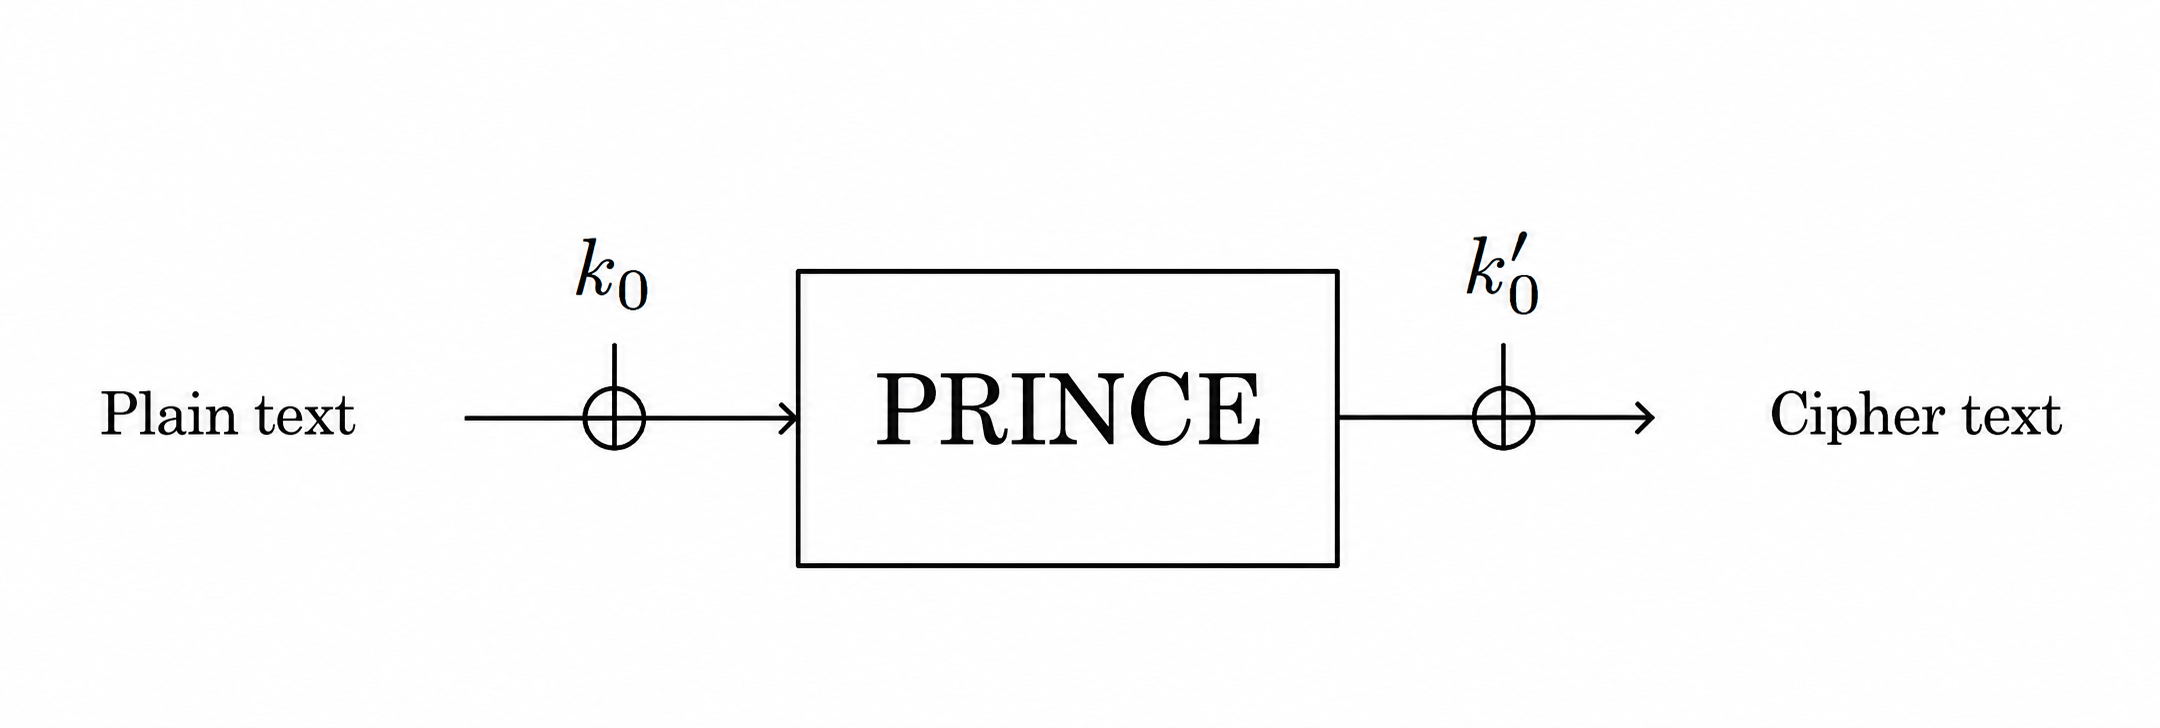
\includegraphics[width= 0.7\textwidth]{Prince_Circuit_Design.png}
\caption{Prince Circuit Design}
\label{fig:Prince_circuit}
\end{figure}

The general structure of the PRINCE algorithm includes whitening initialization, five rounds of processing in the forward direction, a middle layer of processing, five rounds of inverse processing, and the end whitening process. In terms of the master key, which has 128 bits, PRINCE uses two keys $k_0$ and $k_1$, each having 64 bits. At the start of the encryption process, the plaintext data undergoes XOR operation against the key values. For every round in the forward processing procedure, PRINCE performs four major processes: S-layer operation for substitution, M-layer process for diffusion, round constants addition, and round keys addition, utilizing $k_1$. After completing five forward processing rounds, a middle transformation process is performed, followed by five rounds of inverse processing.

\begin{figure}[H]
\centering
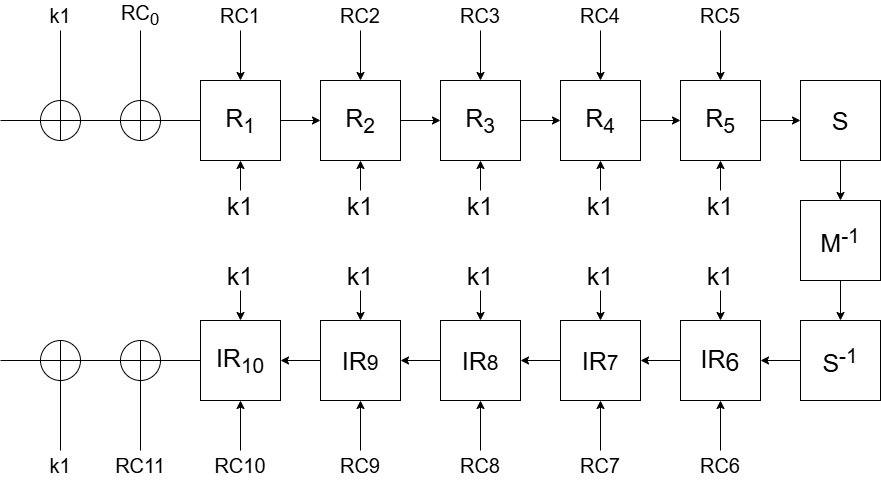
\includegraphics[width=0.85\textwidth]{Prince_Full.png}
\caption{Overall Structure of the PRINCE Block Cipher}
\label{fig:classical_prince_full}
\end{figure}

S-layer constitutes the non-linear substitution layer in PRINCE ciphering algorithm and takes care of the creation of confusion in the algorithm. During this phase, the internal state of 64 bits is broken into sixteen 4-bit nibbles. These 4-bit nibbles are then subjected to substitution transformation independently, which is performed through a defined substitution function called PRINCE S-box. This PRINCE S-box converts every possible 4-bit input to its corresponding 4-bit output, thus not allowing any kind of linear relationship between the plaintext, ciphertext, and the key.

\begin{table}[H]
\centering
\caption{PRINCE S-box Mapping}
\label{tab:classical_prince_sbox}
\begin{tabular}{|c|c|}
\hline
\textbf{Input (Hex)} & \textbf{Output (Hex)} \\
\hline
0x0 & 0xB \\
\hline
0x1 & 0xF \\
\hline
0x2 & 0x3 \\
\hline
0x3 & 0x2 \\
\hline
0x4 & 0xA \\
\hline
0x5 & 0xC \\
\hline
0x6 & 0x9 \\
\hline
0x7 & 0x1 \\
\hline
0x8 & 0x6 \\
\hline
0x9 & 0x5 \\
\hline
0xA & 0x0 \\
\hline
0xB & 0xE \\
\hline
0xC & 0xD \\
\hline
0xD & 0x8 \\
\hline
0xE & 0x4 \\
\hline
0xF & 0x7 \\
\hline
\end{tabular}
\end{table}

The M-layer is the linear diffusion layer of PRINCE and is used to spread the influence of individual bits across the internal state. Its primary objective is to ensure that small changes in the plaintext or key affect many output bits after multiple rounds, thereby improving diffusion. The transformation is represented mathematically using binary matrices over $GF(2)$. The complete 64-bit state is divided into four 16-bit blocks, and each block undergoes a linear transformation using the matrix $M_{16}$. The overall M-layer matrix is therefore constructed as a block diagonal matrix.

\[
I_4 =
\begin{bmatrix}
1 & 0 & 0 & 0 \\
0 & 1 & 0 & 0 \\
0 & 0 & 1 & 0 \\
0 & 0 & 0 & 1
\end{bmatrix}
\qquad
Z_4 =
\begin{bmatrix}
0 & 0 & 0 & 0 \\
0 & 0 & 0 & 0 \\
0 & 0 & 0 & 0 \\
0 & 0 & 0 & 0
\end{bmatrix}
\]

\[
M_{16} =
\begin{bmatrix}
Z_4 & I_4 & I_4 & I_4 \\
I_4 & Z_4 & I_4 & I_4 \\
I_4 & I_4 & Z_4 & I_4 \\
I_4 & I_4 & I_4 & Z_4
\end{bmatrix}
\]

\[
M =
\begin{bmatrix}
M_{16} & 0 & 0 & 0 \\
0 & M_{16} & 0 & 0 \\
0 & 0 & M_{16} & 0 \\
0 & 0 & 0 & M_{16}
\end{bmatrix}_{64 \times 64}
\]

The M-layer performs only linear XOR-based transformations and therefore complements the non-linear behavior introduced by the S-layer. Together, the S-layer and M-layer form the core substitution--permutation structure of the PRINCE cipher.

\section{Reversible Circuits for PRINCE}

This section presents the reversible quantum implementation of the PRINCE block cipher. Since quantum computation requires all operations to be reversible and unitary, the classical PRINCE encryption structure must be transformed into a reversible quantum circuit. The proposed implementation reproduces the behavior of the classical cipher using quantum gates such as Pauli-X, CNOT, and Toffoli gates. Separate quantum registers are used for the plaintext state, key material, and temporary ancilla storage required during reversible computation. The resulting circuit can be embedded into a Grover oracle for quantum key-search applications.

\subsection{Qubit Distribution}

The quantum implementation of PRINCE uses separate qubit registers for storing the plaintext state, secret key components, and ancilla workspace required for reversible operations. The 64-bit state register stores the plaintext and all intermediate values generated during encryption. Additional ancilla qubits are required mainly for reversible S-box computation, where temporary values must be stored without destroying the original input state. Separate registers are also maintained for the key components $k_0$, $k_1$, and the derived key $k_0'$.

\begin{table}[H]
\centering
\caption{Qubit Allocation in Quantum PRINCE Implementation}
\label{tab:qubit_distribution}
\begin{tabular}{|c|c|p{7cm}|}
\hline
\textbf{Qubit Range} & \textbf{Purpose} & \textbf{Description} \\
\hline
0--63 & State Register & Stores the 64-bit plaintext and intermediate cipher state during encryption \\
\hline
64--287 & S-box Ancilla & Ancilla workspace used during reversible implementation of the S-box layer \\
\hline
288--351 & $k_0$ Register & Stores the first 64-bit key half used during initial whitening \\
\hline
352--415 & $k_1$ Register & Stores the round key used in all forward and inverse rounds \\
\hline
416--479 & $k_0'$ Register & Stores the derived key used during final whitening \\
\hline
\end{tabular}
\end{table}

The separation of registers helps preserve reversibility throughout the computation. The ancilla qubits used during intermediate computations are uncomputed back to the $|0\rangle$ state after use, ensuring that no unwanted garbage states remain in the circuit. This property is essential for embedding the encryption circuit into Grover's algorithm, where the oracle must operate reversibly.

\subsection{Quantum Round Structure}

The reversible PRINCE circuit follows the same high-level structure as the classical cipher. The encryption process begins with initial key whitening, followed by five forward rounds, a middle layer, and five inverse rounds. Finally, a last whitening stage is applied using the derived key material.

The inverse rounds apply the inverse transformations in reverse order while preserving reversibility. Since XOR operations are naturally reversible, round-key addition and round constant addition are implemented efficiently using CNOT and Pauli-X gates.

\begin{figure}[H]
\centering
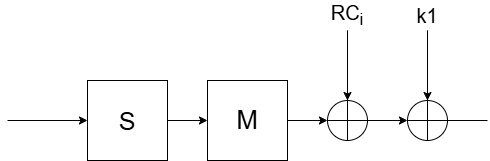
\includegraphics[width=0.65\textwidth]{Forward_Round.png}
\caption{Quantum Forward Round Structure of PRINCE}
\label{fig:quantum_forward_round}
\end{figure}

\begin{figure}[H]
\centering
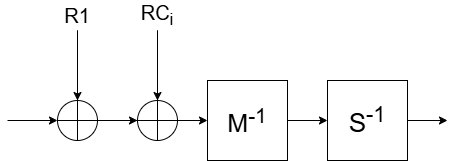
\includegraphics[width=0.65\textwidth]{Backward_Round.png}
\caption{Quantum Inverse Round Structure of PRINCE}
\label{fig:quantum_inverse_round}
\end{figure}

The middle layer connects the forward and inverse halves of the cipher and consists of an S-layer, M-layer, and inverse S-layer. Together, these components preserve the reflection-based structure of PRINCE while remaining compatible with reversible quantum computation.

\subsection{Quantum Key Generation}

The PRINCE key schedule is implemented reversibly using quantum operations. The 128-bit master key is divided into two 64-bit halves, denoted as $k_0$ and $k_1$. A modified key $k_0'$ is generated from $k_0$ using a one-bit circular right rotation followed by XOR with the most significant bit.

\begin{figure}[H]
\centering
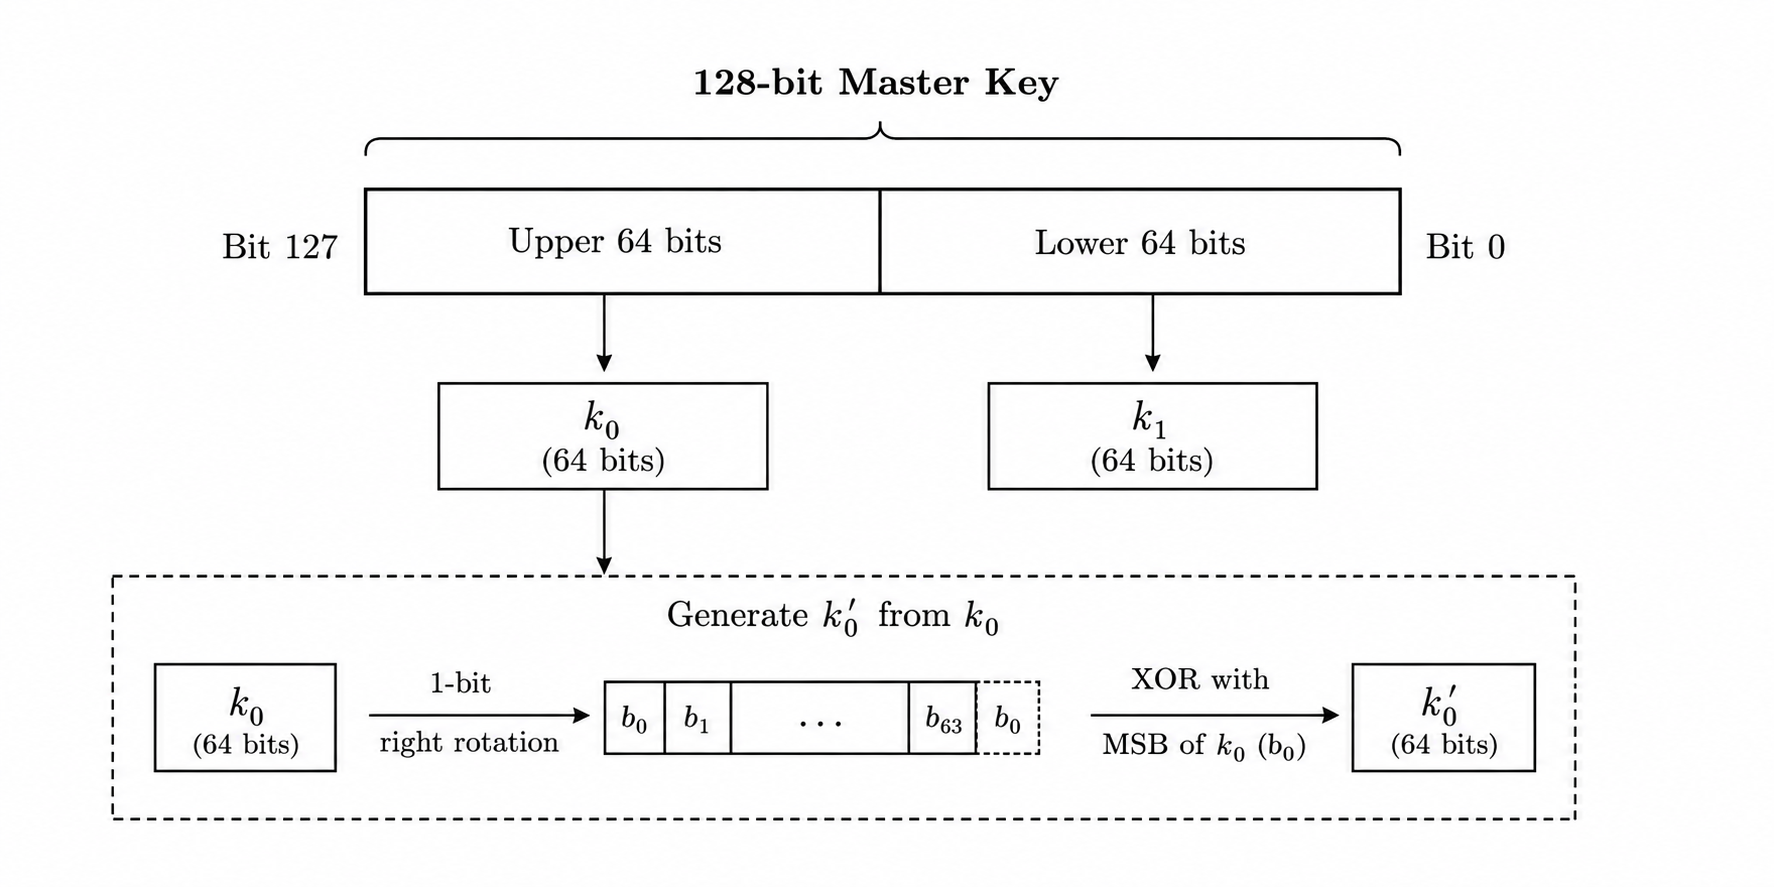
\includegraphics[width=\textwidth]{Key_Generation.png}
\caption{Quantum Key Generation Structure for PRINCE}
\label{fig:quantum_key_generation}
\end{figure}

The generated key material is stored in dedicated quantum registers and reused during the whitening and round-key addition stages. Since the operations used in the key schedule are XOR-based, they can be implemented reversibly using CNOT gates without requiring large additional ancilla resources.

\subsection{Quantum S-box Implementation}

The S-box is the only non-linear component of the PRINCE cipher and therefore represents one of the most important parts of the reversible quantum implementation. In the PRINCE S-layer, the 64-bit state is divided into sixteen 4-bit nibbles, and the same 4-bit substitution is applied independently to each nibble.

Direct lookup-table implementation is not suitable in quantum computation because quantum operations must be reversible and cannot overwrite unknown quantum states. Therefore, the PRINCE S-box is represented using Algebraic Normal Form (ANF), where each output bit is expressed as a combination of XOR terms and product terms over the input bits.

The ANF representation is suitable for quantum implementation because XOR operations can be implemented using CNOT gates. Also, Constant bit flips can be implemented using Pauli-X gates and product terms can be implemented using Toffoli gates

\begin{figure}[h]
\centering
\fbox{
\begin{minipage}{0.92\textwidth}
\setlength{\abovedisplayskip}{3pt}
\setlength{\belowdisplayskip}{3pt}
\begin{align*}
f(a_3,a_2,a_1,a_0)
&= C_0 \oplus C_1a_0 \oplus C_2a_1 \oplus C_3a_0a_1
 \oplus C_4a_2 \oplus C_5a_0a_2 \oplus C_6a_1a_2 \oplus C_7a_0a_1a_2 \\
&\quad \oplus C_8a_3 \oplus C_9a_0a_3 \oplus C_{10}a_1a_3
 \oplus C_{11}a_0a_1a_3 \oplus C_{12}a_2a_3 \\
&\quad \oplus C_{13}a_0a_2a_3 \oplus C_{14}a_1a_2a_3
 \oplus C_{15}a_0a_1a_2a_3 \\[6pt]
& \text{( Follow Möbius transformation
 procedure to get these constansts  )} \\[8pt]
%--- Representative coefficient calculations (b_0) ---
C_0 &= f(0000) = 1 \\
C_1 &= f(0001) \oplus f(0000) = 1 \oplus 1 = 0 \\
C_3 &= f(0011) \oplus f(0010) \oplus f(0001) \oplus f(0000)
     = 0 \oplus 1 \oplus 1 \oplus 1 = 1 \\
C_4 &= f(0100) \oplus f(0000) = 0 \oplus 1 = 1 \\
C_6 &= f(0110) \oplus C_0 \oplus C_2 \oplus C_4
     = 1 \oplus 1 \oplus 0 \oplus 1 = 1 \\
C_8 &= f(1000) \oplus f(0000) = 0 \oplus 1 = 1 \\
&\quad \vdots \quad \text{(remaining } C_i \text{ computed similarly; } C_{10}=C_{11}=\cdots=C_{15}=0 \text{)} \\[8pt]
%--- Final ANF equations for all output bits ---
b_0 &= 1
  \oplus a_0a_1
  \oplus a_2
  \oplus a_1a_2
  \oplus a_0a_1a_2
  \oplus a_3
  \oplus a_0a_3 \\[4pt]
b_1 &= 1
  \oplus a_0a_2
  \oplus a_1a_2
  \oplus a_0a_1a_2
  \oplus a_0a_3
  \oplus a_1a_3
  \oplus a_2a_3 \\[4pt]
b_2 &= a_0
  \oplus a_0a_1
  \oplus a_3
  \oplus a_0a_3
  \oplus a_1a_3
  \oplus a_0a_2a_3
  \oplus a_1a_2a_3 \\[4pt]
b_3 &= 1
  \oplus a_1
  \oplus a_1a_2
  \oplus a_0a_1a_2
  \oplus a_3
  \oplus a_1a_3
  \oplus a_0a_1a_3
  \oplus a_2a_3
\end{align*}
\end{minipage}
}
\caption{ANF coefficient calculation (representative steps for $b_0$) and final ANF equations for all PRINCE S-box output bits}
\label{fig:anf_combined}
\end{figure}

The resulting reversible S-box circuit is implemented using a combination of Pauli-X, CNOT, and Toffoli gates. Temporary ancilla qubits are used during intermediate computations and are later uncomputed to maintain reversibility.

\begin{table}[H]
\centering
\caption{Quantum Resource Requirement for One PRINCE S-layer}
\label{tab:sbox_resource}
\begin{tabular}{|c|c|p{7cm}|}
\hline
\textbf{Resource} & \textbf{Count} & \textbf{Description} \\
\hline
S-box Instances & 16 & One S-box is applied independently to each 4-bit nibble of the 64-bit state \\
\hline
Input Qubits & 64 & State qubits used as input to the S-layer \\
\hline
Ancilla Qubits & 224 & Temporary workspace qubits required for reversible ANF computation \\
\hline
Pauli-X Gates & 80 & Used for constant bit flips in the ANF implementation \\
\hline
CNOT Gates & 880 & Used for XOR operations in the reversible S-box computation \\
\hline
Toffoli Gates & 640 & Used for implementing non-linear product terms in the ANF equations \\
\hline
Total Quantum Gates & 1600 & Total number of gates required for one complete S-layer \\
\hline
\end{tabular}
\end{table}

\begin{figure}[H]
\centering
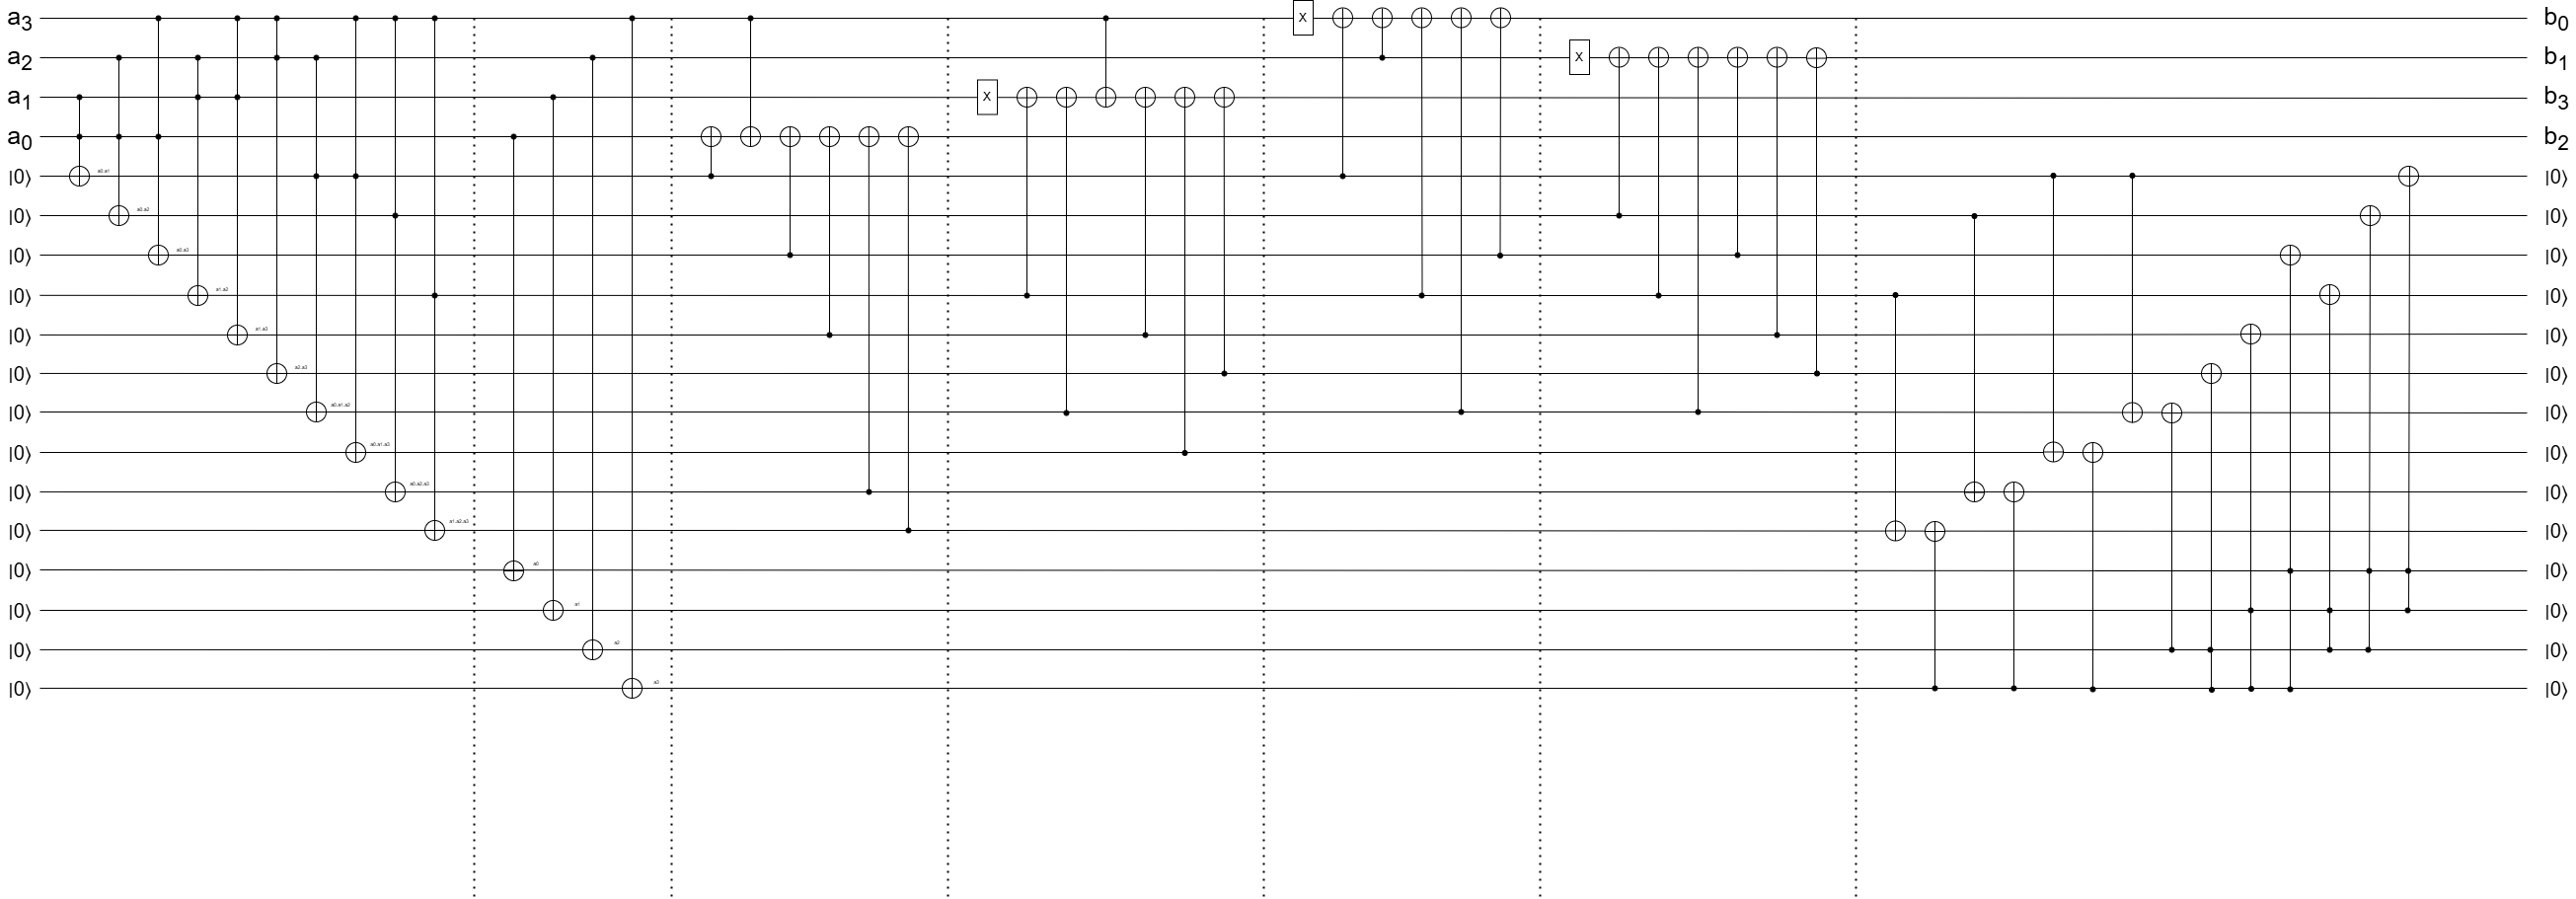
\includegraphics[width=\linewidth]{S-nibble.png}
\caption{Reversible Quantum Circuit for the PRINCE S-box}
\label{fig:quantum_sbox_circuit}
\end{figure}

The PRINCE S-layer operates on the complete 64-bit internal state by dividing it into sixteen independent 4-bit nibbles. Each nibble is processed using the reversible ANF-based S-box circuit. Since the same S-box structure is reused for all sixteen nibbles, the total resource requirement of one S-layer is obtained by multiplying the resource cost of a single S-box by sixteen. The S-layer contributes significantly to the overall quantum resource cost of the PRINCE circuit because the non-linear ANF terms require a large number of Toffoli gates and ancilla qubits.



\begin{figure}[h]
\centering
\fbox{
\begin{minipage}{0.88\textwidth}
\setlength{\abovedisplayskip}{3pt}
\setlength{\belowdisplayskip}{3pt}
\begin{align*}
y &= Mx, \qquad M \in GF(2)^{64 \times 64} \\[2pt]
R_i &\leftarrow R_i \oplus R_j
\end{align*}

Over $GF(2)$, adding row $R_j$ to row $R_i$ is the same as XORing the
corresponding values. In a quantum circuit, this row operation is implemented as:

\[
\text{CNOT}(q_j, q_i): \quad q_i \leftarrow q_i \oplus q_j
\]

Gaussian elimination reduces the matrix $M$ to the identity matrix:

\[
E_t E_{t-1} \cdots E_2 E_1 M = I
\]

where each $E_i$ is an elementary row-operation matrix. Therefore,

\[
M = E_1^{-1} E_2^{-1} \cdots E_{t-1}^{-1} E_t^{-1}
\]

Since XOR row operations are self-inverse over $GF(2)$,

\[
E_i^{-1} = E_i
\]

Hence,

\[
M = E_1 E_2 \cdots E_t
\]
\end{minipage}
}
\caption{Gaussian elimination method for in-place M-box implementation}
\label{fig:gaussian_mbox}
\end{figure}


\subsection{Quantum M-box Implementation}

The M-box is the linear diffusion layer of the PRINCE cipher and is responsible for spreading bit changes across the internal state. Unlike the S-box, the M-box contains only linear XOR-based operations and can therefore be implemented efficiently using CNOT gates. 

The M-layer is represented mathematically using binary matrices over $GF(2)$. The complete 64-bit transformation is constructed using repeated $16 \times 16$ diffusion blocks. 


A direct implementation of the matrix multiplication would require additional workspace qubits. To reduce ancilla usage, the M-box is implemented in-place using Gaussian elimination over $GF(2)$, mathematical proof of this is shown at Figure \ref{fig:gaussian_mbox}. In this method, each elementary row operation corresponds directly to a CNOT gate, allowing the linear transformation to be realized reversibly without allocating a separate output register.

\begin{figure}[H]
\centering

\includegraphics[width=\linewidth]{Mbox.png}
\caption{Quantum Circuit Implementation of the PRINCE M-box}
\label{fig:quantum_mbox}
\end{figure}

\begin{table}[H]
\centering
\caption{Quantum Resource Requirement for One PRINCE M-layer}
\label{tab:mbox_resource}
\begin{tabular}{|c|c|p{7cm}|}
\hline
\textbf{Resource} & \textbf{Count} & \textbf{Description} \\
\hline
Input Qubits & 64 & State qubits representing the 64-bit PRINCE internal state \\
\hline
Ancilla Qubits & 0 & The M-layer is implemented in-place without requiring additional ancilla qubits \\
\hline
Pauli-X Gates & 0 & No constant bit inversions are required in the linear diffusion layer \\
\hline
CNOT Gates & 224 & Used to realize the linear matrix transformation through Gaussian elimination \\
\hline
Toffoli Gates & 0 & The M-layer contains only linear XOR operations and therefore requires no non-linear gates \\
\hline
Total Quantum Gates & 224 & Total number of quantum gates required for one complete M-layer \\
\hline
\end{tabular}
\end{table}

The PRINCE M-layer is implemented as a reversible linear transformation over the 64-bit internal state. Since the transformation contains only XOR-based operations, the complete circuit can be realized entirely using CNOT gates. To avoid the use of additional output registers, the matrix operation is implemented in-place using Gaussian elimination over $GF(2)$. Each elementary row operation corresponds directly to a CNOT gate, allowing the M-layer to be implemented efficiently without requiring ancilla qubits or non-linear Toffoli gates.


\subsection{Round-wise Gate Distribution}

The gate count of the PRINCE circuit is analyzed round by round. Each forward and inverse round contains an S-layer, M-layer, round constant addition, and key addition. The number of CNOT and Toffoli gates remains fixed for each round, while the number of X gates changes depending on the Hamming weight of the round constant.

\begin{table}[h]
\centering
\caption{Round-wise Gate Distribution of PRINCE}
\label{tab:round_gate_distribution}
\begin{tabular}{|c|c|c|c|c|}
\hline
\textbf{Stage} & \textbf{X Gates} & \textbf{CNOT Gates} & \textbf{Toffoli Gates} & \textbf{Total Gates} \\
\hline
Initial Key Addition & 0 & 128 & 0 & 128 \\
\hline
Round 1 & 105 & 1168 & 640 & 1913 \\
\hline
Round 2 & 105 & 1168 & 640 & 1913 \\
\hline
Round 3 & 110 & 1168 & 640 & 1918 \\
\hline
Round 4 & 107 & 1168 & 640 & 1915 \\
\hline
Round 5 & 113 & 1168 & 640 & 1921 \\
\hline
Middle Layer & 160 & 1984 & 1280 & 3424 \\
\hline
Inverse Round 6 & 119 & 1168 & 640 & 1927 \\
\hline
Inverse Round 7 & 105 & 1168 & 640 & 1913 \\
\hline
Inverse Round 8 & 108 & 1168 & 640 & 1916 \\
\hline
Inverse Round 9 & 107 & 1168 & 640 & 1915 \\
\hline
Inverse Round 10 & 111 & 1168 & 640 & 1919 \\
\hline
Final Whitening & 32 & 128 & 0 & 160 \\
\hline
\textbf{Total} & \textbf{1282} & \textbf{13920} & \textbf{7680} & \textbf{22882} \\
\hline
\end{tabular}
\end{table}

\section{Resource Estimation under Parallelism}

Grover's algorithm provides a quadratic speedup for exhaustive key search, but a complete Grover search over the full PRINCE key space still requires a very large sequential circuit depth. One way to reduce the required depth is to use \textbf{inner parallelization}. The machines do not cooperate during a Grover iteration; instead, each machine runs Grover search on a smaller portion of the key space.

Let the PRINCE key size be $k=128$. The full key space has size $2^k$. Assume that one Grover iteration for the PRINCE oracle has gate cost $O_g$ and circuit depth $O_d$. If $M=2^m$ quantum machines are used in parallel, then each machine searches only $2^{k-m}$ keys. Therefore, the approximate number of Grover iterations required per machine is
\[
I_m \approx \frac{\pi}{4}\sqrt{2^{k-m}}
      = \frac{\pi}{4}2^{(k-m)/2}.
\]

The depth required by each parallel machine is then
\[
D_m = I_m O_d
    \approx \frac{\pi}{4}2^{(k-m)/2}O_d.
\]
Thus, increasing the number of machines decreases the depth of the computation on each machine. However, this does not reduce the total work. Since all $M=2^m$ machines run their own Grover search, the total gate cost over all machines is
\[
G_m = 2^m I_m O_g
    \approx \frac{\pi}{4}2^{(k+m)/2}O_g.
\]

If a maximum allowed circuit depth $D_{\max}$ is fixed, the required number of parallel machines can be estimated by solving $D_m = D_{\max}$. This gives
\[
M = 2^m
  \approx
  \left(\frac{\pi}{4}\right)^2
  \frac{2^k O_d^2}{D_{\max}^2}.
\]
Substituting this value into the total gate cost gives the total depth-limited gate cost
\[
G_{D_{\max}}
  \approx
  \left(\frac{\pi}{4}\right)^2
  \frac{2^k O_g O_d}{D_{\max}}.
\]

For the PRINCE Grover circuit constructed in this work, the optimized one-iteration resources are
\[
O_g = 46806,\qquad O_d = 2015.
\]
Using these values, Table~\ref{tab:parallel_resource_prince} shows the estimated number of parallel machines and total gate cost for selected depth limits. The values are expressed as powers of two because the quantities are extremely large.

\begin{table}[H]
\centering
\caption{Depth-Limited Parallel Resource Estimate for PRINCE Grover Search}
\label{tab:parallel_resource_prince}
\small
\renewcommand{\arraystretch}{1.3}

\begin{tabular}{|
>{\centering\arraybackslash}m{2.5cm}|
>{\centering\arraybackslash}m{2.8cm}|
>{\centering\arraybackslash}m{3.2cm}|
>{\centering\arraybackslash}m{4.5cm}|
}
\hline

\textbf{\shortstack{Depth Limit\\$D_{\max}$}} &
\textbf{\shortstack{Parallel\\Machines $M$}} &
\textbf{\shortstack{Total Gate\\Cost $G_{D_{\max}}$}} &
\textbf{Interpretation} \\
\hline

$2^{40}$ &
$\approx 2^{69.26}$ &
$\approx 2^{113.79}$ &
Very high parallelism is required to satisfy a shallow depth bound. \\
\hline

$2^{64}$ &
$\approx 2^{21.26}$ &
$\approx 2^{89.79}$ &
Fewer machines are needed, but the total gate cost remains large. \\
\hline

\end{tabular}
\end{table}
This analysis shows the main trade-off in parallel Grover search. Parallelism reduces the circuit depth required on each individual quantum machine, but it increases the total hardware requirement because many machines must be available at the same time. For PRINCE, even with parallelization, the total resource requirement remains very large. Therefore, the practical difficulty of a Grover-based attack is not only the number of Grover iterations, but also the combined cost of qubits, gates, depth, and the number of parallel quantum machines required.

\cleardoublepage
\onehalfspacing

%------------ Chapter 5--------------------------------

\cleardoublepage
\onehalfspacing







\chapter{Implementation Details and Setup}

This chapter presents the practical aspects of the implementation of the reversible quantum Prince circuit and the Grover-based key search attack. It details the tools, libraries, and simulation environment used to build and run the quantum circuits, together with the assumptions and constraints considered during the implementation. The chapter also outlines design choices made to adapt to hardware and memory limitations, including a reduced key space for Grover's algorithm.

\subsection{Software Configuration}

The following is a summary of the software environment used for implementation:
\begin{itemize}
\item Programming Language: Python 3.10
\item Quantum Computing Framework: Qiskit SDK for quantum circuit design and simulation
\item Numerical Computing Libraries: NumPy, Pandas
\item Data Visualization Tools: Matplotlib, Seaborn
\item Development and Execution Platform: Jupyter Notebook and Google Colab
\end{itemize}

\subsection{Hardware Configuration}

The experiments were performed using a system with the following configuration:
\begin{itemize}
\item Processor: AMD Ryzen 9 CPU
\item Graphics Processing Unit: NVIDIA GeForce RTX 2060
\item System Memory: 16 GB RAM
\item Type of Environment: Full software quantum simulation
\end{itemize}

\subsection{Simulation Constraints}

The complete PRINCE-based Grover attack uses a 128-bit key register, which means that a full quantum simulation would require representing a superposition over $2^{128}$ possible keys. This is far beyond the memory and computational capacity of classical quantum simulators. Therefore, the full Grover attack is not simulated directly in this work. Instead, the PRINCE encryption circuit is verified separately for correctness, and the Grover iteration circuit is constructed for resource estimation. This allows the qubit count, gate count, circuit depth, T-gate count, and T-depth to be evaluated without attempting an infeasible full-state simulation.


\section{Evaluation Metrics}

For evaluating the proposed quantum PRINCE implementation and the Grover-based key search circuit, resource estimation is used as the main evaluation method. Since the full 128-bit Grover attack cannot be simulated on classical hardware, the analysis focuses on circuit-level metrics that indicate the cost and feasibility of the quantum implementation. The results include the total number of qubits, total gate count, gate-wise distribution, and logical circuit depth for the PRINCE encryption circuit and for one Grover iteration. In addition, Clifford+T resource metrics are reported, including the total number of Clifford gates, total number of T gates, T-depth, and total Clifford+T depth. 




\chapter{RESULTS AND DISCUSSION}

\section{Correctness Verification}

The correctness of the proposed quantum PRINCE implementation is verified by comparing the ciphertext obtained from the classical PRINCE implementation with the ciphertext obtained from the quantum circuit. For the same plaintext and key, both implementations must produce the same ciphertext. The results in Table~\ref{tab:classical_quantum_match} show that the quantum implementation correctly reproduces the classical PRINCE encryption.

\begin{table}[h]
\centering
\caption{Classical and Quantum PRINCE Ciphertext Comparison}
\label{tab:classical_quantum_match}
\resizebox{\textwidth}{!}{%
\begin{tabular}{|c|c|c|c|}
\hline
\textbf{Plaintext} & \textbf{Key} & \textbf{Classical Ciphertext} & \textbf{Quantum Ciphertext} \\
\hline
0x0000000000000000 & 0x00000000000000000000000000000000 & 0xB607FA70A2065323 & 0xB607FA70A2065323 \\
\hline
0x1111111111111111 & 0x0ABCDEFFEDC123456789BA9876543210 & 0x44FBFF21F4BA60E1 & 0x44FBFF21F4BA60E1 \\
\hline
\end{tabular}
}
\end{table}

PRINCE has a special property known as alpha reflection. This property allows decryption to be performed using a closely related structure to encryption by modifying the key material. In this work, the ciphertext obtained from encryption is again passed through the decryption structure using the alpha-reflection relation. The output matches the original plaintext, confirming that the implemented forward and inverse structures are consistent.

\begin{table}[h]
\centering
\caption{Alpha Reflection Verification}
\label{tab:alpha_reflection}
\begin{tabular}{|c|c|c|c|}
\hline
\textbf{Plaintext} & \textbf{Ciphertext} & \textbf{Recovered Plaintext} & \textbf{Result} \\
\hline
0x1111111111111111 & 0x44FBFF21F4BA60E1 & 0x1111111111111111 & PASS \\
\hline
\end{tabular}
\end{table}

\section{Clifford Decomposition}

To estimate fault-tolerant quantum resources, the PRINCE circuit is decomposed into Clifford and T gates. In this decomposition, Clifford gates include gates such as X, H, S, and CNOT, while the T gate is treated as an expensive non-Clifford resource. The Toffoli gates in the PRINCE circuit are decomposed into Clifford+T form, and the resulting Clifford gate count, T-gate count, T-depth, and total depth are recorded.

\begin{table}[H]
\centering
\caption{Clifford+T Resource Estimation for Efficient PRINCE}
\label{tab:clifford_prince}
\begin{tabular}{|c|c|c|c|c|}
\hline
\textbf{Qubits} & \textbf{Clifford Gates} & \textbf{T Gates} & \textbf{T-depth} & \textbf{Total Depth} \\
\hline
480 & 69218 & 53760 & 1560 & 4269 \\
\hline
\end{tabular}
\end{table}


\begin{figure}[h]
\centering
\fbox{
\begin{minipage}{0.92\textwidth}
\setlength{\abovedisplayskip}{3pt}
\setlength{\belowdisplayskip}{3pt}

\textbf{Mathematical Gate Count for One Grover Iteration}

\begin{align*}
\textbf{Plaintext loading:}\qquad
X &= 16 \\[3pt]
\textbf{Key superposition:}\qquad
H &= 128 \\[3pt]
\textbf{Compute and uncompute } k_0':\qquad
CNOT &= 65 + 65 = 130
\end{align*}

\begin{align*}
\textbf{PRINCE encryption + uncomputation:}\qquad
X &= 2 \times 1282 = 2564, \\
CNOT &= 2 \times 13920 = 27840, \\
Toffoli &= 2 \times 7680 = 15360
\end{align*}

\begin{align*}
\textbf{Ciphertext phase marker:}\qquad
X &= 2 \times 35 + 128 = 198, \\
Toffoli &= 126, \\
Z &= 1
\end{align*}

\begin{align*}
\textbf{128-bit diffuser:}\qquad
H &= 2 \times 128 = 256, \\
X &= 2 \times 128 = 256, \\
Toffoli &= 254, \\
Z &= 1
\end{align*}

\begin{align*}
\textbf{Total one Grover iteration:}\qquad
H &= 128 + 256 = 384, \\
X &= 16 + 2564 + 198 + 256 = 3034, \\
CNOT &= 27840 + 130 = 27970, \\
Toffoli &= 15360 + 126 + 254 = 15740, \\
Z &= 1 + 1 = 2, \\
Total &= 384 + 3034 + 2 + 27970 + 15740 \\
Total &= 47130
\end{align*}

\end{minipage}
}
\caption{Mathematical gate count calculation for one Grover iteration}
\label{fig:math_grover_calc}
\end{figure}


\section{One Grover Iteration}

A single Grover iteration is constructed using the PRINCE encryption circuit as the oracle. The key register is placed in superposition, the encryption circuit is applied, the matching ciphertext is phase-marked, and the encryption is then uncomputed before applying the Grover diffuser. However, simulating the complete Grover attack is not possible on classical hardware because the 128-bit key register would require representing $2^{128}$ possible key states. Therefore, the Grover circuit is constructed only for resource estimation.

In the actual Qiskit implementation, some X gates are automatically cancelled during optimization. Therefore, the manually calculated X gate count is slightly higher than the optimized circuit count. The CNOT, Toffoli, H, and Z gate counts remain the same, while the optimized total gate count becomes smaller.

\begin{table}[H]
\centering
\caption{Mathematical and Actual Gate Count Comparison}
\label{tab:math_actual_comparison}
\begin{tabular}{|c|c|c|c|c|c|c|}
\hline
\textbf{Method} & \textbf{H} & \textbf{X} & \textbf{Z} & \textbf{CNOT} & \textbf{Toffoli} & \textbf{Total} \\
\hline
Manual Calculation & 384 & 3034 & 2 & 27970 & 15740 & 47130 \\
\hline
Qiskit Optimized & 384 & 2710 & 2 & 27970 & 15740 & 46806 \\
\hline
\end{tabular}
\end{table}

\section{Overall Resource Summary}

Table~\ref{tab:overall_results} summarizes the main results obtained in this work. The normal PRINCE circuit provides the basic reversible implementation, while the Clifford decomposition gives the corresponding fault-tolerant resource estimate. Similarly, one Grover iteration is constructed and then decomposed into Clifford+T resources.

\begin{table}[H]
\centering
\caption{Overall Resource Estimation Results}
\label{tab:overall_results}
\small
\begin{tabularx}{\textwidth}{|X|c|c|c|c|c|}
\hline
\textbf{Circuit} & \textbf{Qubits} & \textbf{Total Gates} & \textbf{Depth} & \textbf{T Gates} & \textbf{T-depth} \\
\hline
Normal PRINCE & 480 & 22882 & 10712 & -- & -- \\
\hline
PRINCE with Clifford Decomposition & 480 & -- & 4269 & 53760 & 1560 \\
\hline
One Grover Iteration & 607 & 46806 & 2015 & -- & -- \\
\hline
One Grover Iteration with Clifford Decomposition & 607 & -- & 11963 & 110180 & 4452 \\
\hline
\end{tabularx}
\end{table}
    

\chapter{Toy PRINCE}

The complete PRINCE Grover circuit cannot be simulated over the full 128-bit key space on a classical machine. To demonstrate the same idea end-to-end, a reduced cipher named \textbf{Toy PRINCE} was implemented. The purpose of this toy construction is not to replace PRINCE, but to provide a small model in which the encryption function, alpha-reflection property, oracle marking, Grover amplitude amplification, and final key recovery can all be verified by direct simulation.

\begin{table}[H]
\centering
\caption{Toy PRINCE Design Parameters}
\label{tab:toy_prince_parameters}
\begin{tabularx}{\textwidth}{|X|c|X|}
\hline
\textbf{Component} & \textbf{Size / Value} & \textbf{Role in the Toy Cipher} \\
\hline
State register & 4 bits & Stores one nibble of plaintext, intermediate state, and ciphertext \\
\hline
Key register & 8 bits & Search space for Grover key recovery, divided as $k_0 || k_1$ \\
\hline
S-box & 4-bit PRINCE S-box & Provides the non-linear substitution layer \\
\hline
M-box & 4-bit involution & Provides reversible linear diffusion \\
\hline
Alpha constant & 0x8 & Flips the high bit of $k_1$ and switches the core between forward and inverse operation \\
\hline
Search space & $2^8 = 256$ keys & Small enough for full state-vector Grover simulation \\
\hline
\end{tabularx}
\end{table}


Toy PRINCE uses a 4-bit state and an 8-bit key. The 8-bit key is divided into two 4-bit halves, $k_0$ and $k_1$, and a derived key $k_0'$ is generated from $k_0$ in the same spirit as the PRINCE key schedule. The PRINCE 4-bit S-box is reused directly, because the complete toy state is one nibble. A small involutive 4-bit M-box is used as the linear diffusion layer, so that applying the M-box twice gives the identity. The round constants are reduced to three 4-bit constants:
\[
RC_0 = 0,\qquad RC_1 = 7,\qquad RC_2 = D.
\]


The implemented encryption structure is
\[
C = F_{k_1}(P \oplus k_0 \oplus RC_0) \oplus k_0',
\]
where $F_{k_1}$ is the toy PRINCE core. The core applies two reduced rounds:
\[
R_1 = AddKeyConst(k_1,RC_1) \rightarrow S \rightarrow M,
\]
\[
R_2 = AddKeyConst(rotl(k_1),RC_2) \rightarrow S \rightarrow M.
\]
The high bit of $k_1$ is reserved for alpha reflection. If this bit is set, the core applies the inverse round order. Therefore,
\[
F_{k_1 \oplus \alpha}(F_{k_1}(x)) = x,
\]
where $\alpha = 0x8$. This reproduces the central idea of PRINCE alpha reflection at a scale where every key and plaintext can be exhaustively checked.

\begin{figure}[H]
\centering
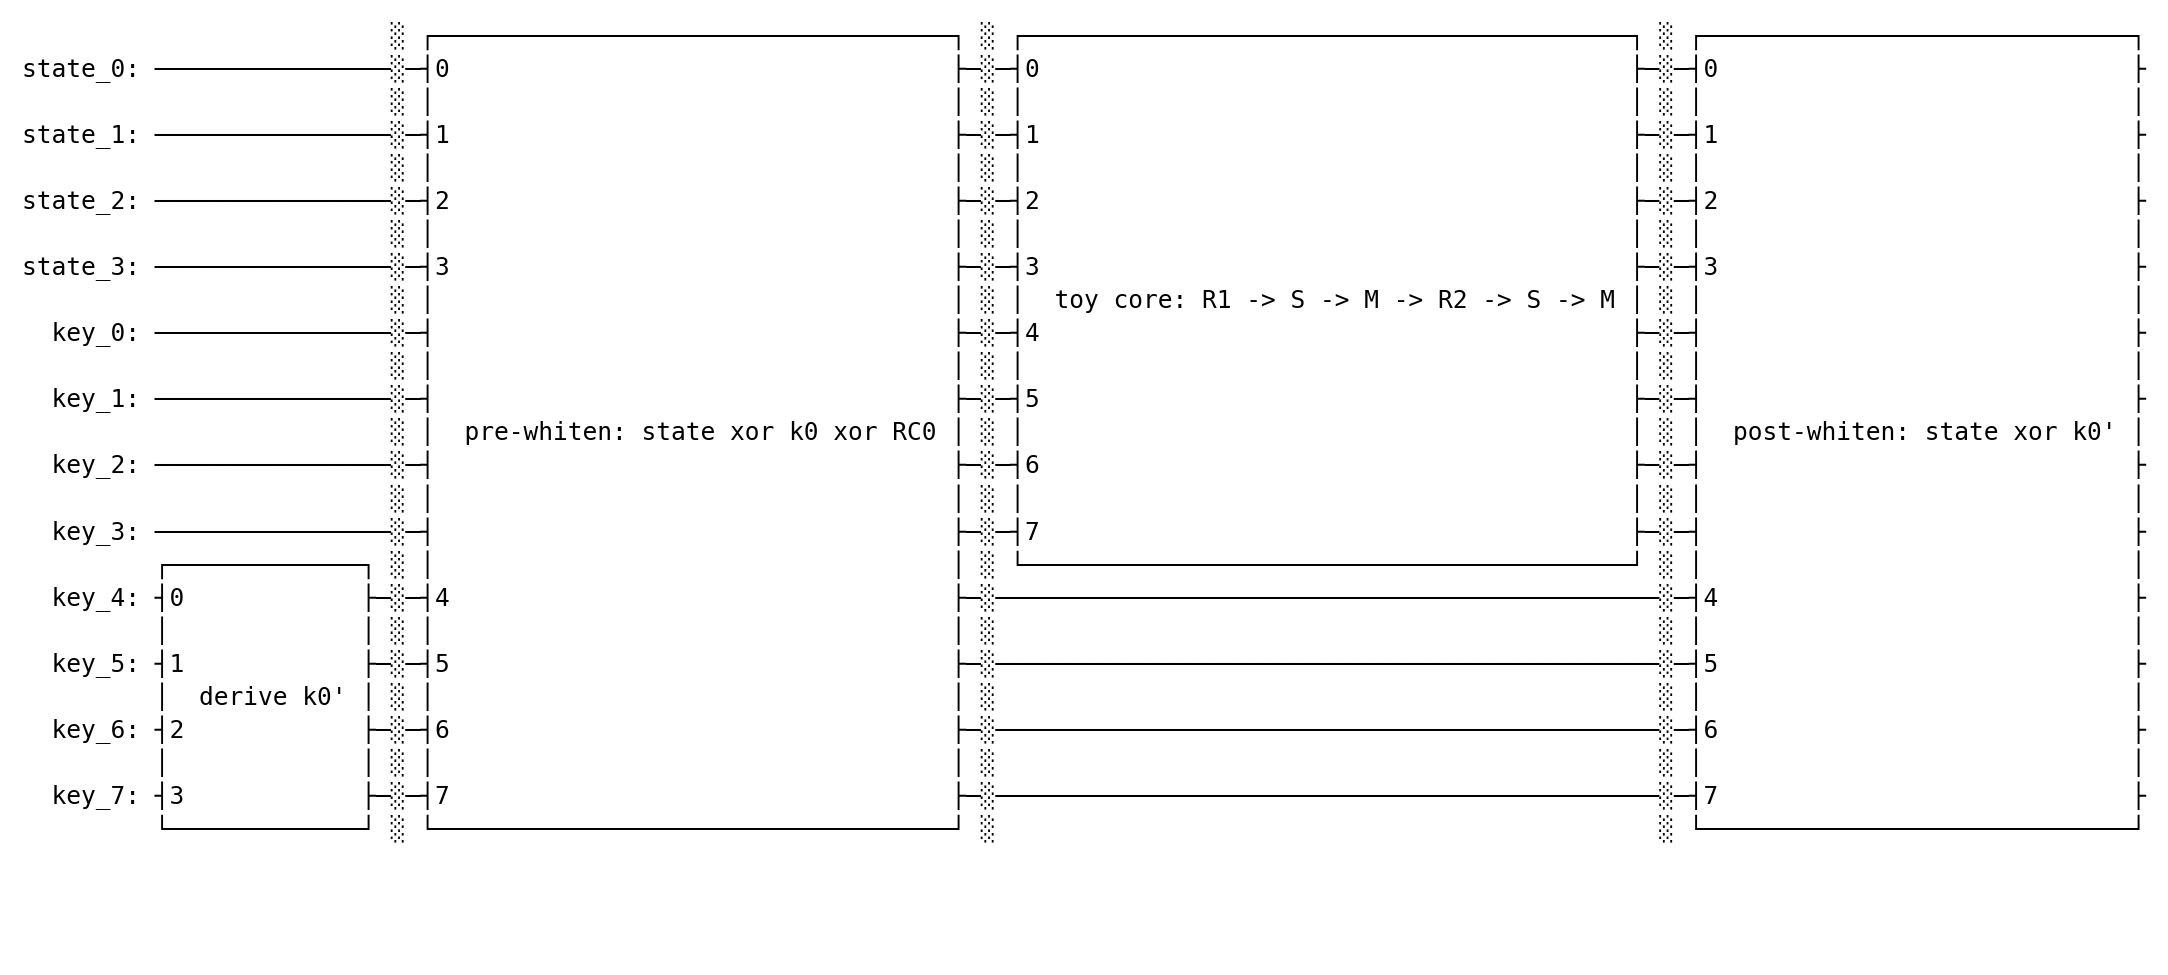
\includegraphics[width=\textwidth]{toy_prince_full_circuit.png}
\caption{Block-level circuit representation of Toy PRINCE encryption}
\label{fig:toy_prince_full_circuit}
\end{figure}

The Toy PRINCE implementation was first verified classically. The zero test confirms that the encryption and decryption routines are mutually consistent. A non-zero test uses plaintext $0x9$ and key $0x6D$, for which the key schedule gives $k_0=0x6$, $k_1=0xD$, and $k_0'=0x3$. The resulting ciphertext is $0x2$. In addition, every one of the 256 possible keys was checked over all 16 plaintext values to confirm that encryption is a permutation and that decryption recovers the original plaintext.

\begin{table}[H]
\centering
\caption{Toy PRINCE Correctness Verification}
\label{tab:toy_prince_correctness}
\small
\begin{tabularx}{\textwidth}{|X|c|c|c|c|}
\hline
\textbf{Test} & \textbf{Plaintext} & \textbf{Key} & \textbf{Ciphertext} & \textbf{Result} \\
\hline
Zero encrypt/decrypt & 0x0 & 0x00 & 0xB & PASS \\
\hline
Non-zero encrypt/decrypt & 0x9 & 0x6D & 0x2 & PASS \\
\hline
Reversibility & All 16 plaintexts & All 256 keys & -- & PASS \\
\hline
Alpha reflection & All 16 states & All 16 $k_1$ values & -- & PASS \\
\hline
\end{tabularx}
\end{table}

After correctness verification, Toy PRINCE was embedded in a Grover key-search experiment. The secret key was fixed as $0x6D$. Three known plaintext--ciphertext pairs were generated from this key and used by the oracle. The use of three pairs removes false key candidates in the 8-bit search space, leaving exactly one marked key.

\begin{table}[H]
\centering
\caption{Known Plaintext--Ciphertext Pairs Used in Toy PRINCE Grover Search}
\label{tab:toy_prince_known_pairs}
\begin{tabular}{|c|c|c|}
\hline
\textbf{Pair} & \textbf{Plaintext} & \textbf{Ciphertext under key 0x6D} \\
\hline
1 & 0x9 & 0x2 \\
\hline
2 & 0x2 & 0x4 \\
\hline
3 & 0xE & 0x3 \\
\hline
\end{tabular}
\end{table}

The Grover simulation starts with a uniform superposition over all 256 keys, so each key initially has probability $1/256 = 0.003906$. The oracle flips the phase of key $0x6D$, and the diffuser then amplifies its amplitude. The simulation was stopped when the highest key probability crossed the selected threshold of $0.99$. The correct key reached probability $0.999947$ after 12 Grover iterations.

\begin{table}
\centering
\caption{Toy PRINCE Grover Probability Amplification}
\label{tab:toy_prince_grover_summary}
\small
\begin{tabularx}{\textwidth}{|c|c|X|X|}
\hline
\textbf{Iteration} & \textbf{Most Probable Key} & \textbf{Top Key Probability} & \textbf{Marked-Key Probability} \\
\hline
0 & 0x00 & 0.003906 & 0.003906 \\
\hline
1 & 0x6D & 0.034791 & 0.034791 \\
\hline
4 & 0x6D & 0.284743 & 0.284743 \\
\hline
8 & 0x6D & 0.763722 & 0.763722 \\
\hline
10 & 0x6D & 0.935176 & 0.935176 \\
\hline
11 & 0x6D & 0.982583 & 0.982583 \\
\hline
12 & 0x6D & 0.999947 & 0.999947 \\
\hline
\end{tabularx}
\end{table}

\begin{figure}
\centering

\includegraphics[width=\textwidth]{toy_prince_grover_attack_full_circuit.png}
\caption{Block-level circuit for one Toy PRINCE Grover attack iteration}
\label{fig:toy_prince_grover_full_circuit}
\end{figure}

The Toy PRINCE experiment confirms the complete workflow used for the main PRINCE study. First, a PRINCE-like reversible cipher is defined using key whitening, S-box substitution, an M-layer, round constants, and a derived whitening key. Second, the cipher is verified for reversibility and alpha reflection. Third, the encryption circuit is used inside an oracle that marks keys consistent with known plaintext--ciphertext pairs. Finally, Grover diffusion amplifies the marked key until it dominates the measurement distribution. This small-scale experiment demonstrates the full attack mechanism that is infeasible to simulate directly for the 128-bit PRINCE key space.

\begin{figure}[h]
    \centering
    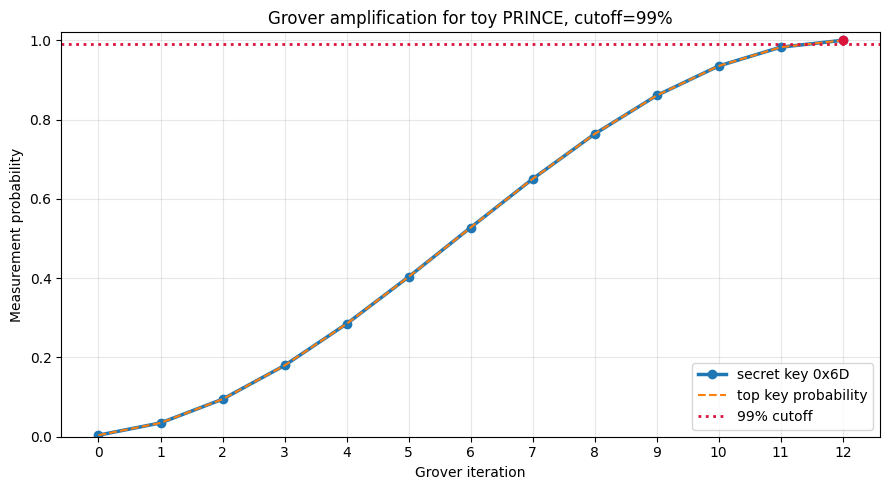
\includegraphics[width=0.65\linewidth]{Grover-amplification.png}
    \caption{Grover amplification}
    \label{fig:GroverAmplification}
\end{figure}

\chapter{Conclusion and Future Work}

This thesis presented a reversible quantum implementation of the PRINCE lightweight block cipher and analyzed its use within a Grover-based key search framework. A complete reversible circuit for the PRINCE encryption structure was constructed by implementing the S-box layer, M-layer, round constants, key addition operations, and the PRINCE key schedule using reversible quantum operations. The resulting circuit preserves the functional behavior of the classical PRINCE cipher while satisfying the reversibility requirements of quantum computation.

The project also showed how reversible PRINCE circuit can be implemented within the oracle circuit of the Grover algorithm to enable the quantum exhaustive search for cryptographic keys. A single Grover iteration was implemented with oracle computation, phase inversion, uncomputation, and Grover diffuser. However, as a full simulation over the whole 128-bit space of the keys would involve $2^{128}$ states, a full-state simulation was not possible on classical computer. Hence, the project concentrated on designing a circuit and evaluating its correctness and resources.

Correctness was proven by testing the equivalence between the output of the classic and quantum PRINCE implementations, as well as by demonstrating the alpha-reflection properties of PRINCE. The next step in the research was a resource analysis for the quantum PRINCE encryption circuit and a single Grover iteration. Such metrics as number of qubits, total gate count, number of layers in the circuit, number of Clifford gates, T gates, and T-depth were calculated. As it turns out, although Grover's algorithm enables an attacker to reduce the security level of a 128-bit key to 64 bits from a theoretical standpoint, its realization involves a huge number of gates, circuit depth, and fault-tolerant resources.

This work emphasizes that while there have been many theoretical studies on the ability of quantum search algorithms to break symmetric block ciphers, they do not take into account the complexities of such an operation on a practical scale. This study further proves that the post-quantum strength of symmetric block ciphers can be analyzed by designing a reversible circuit and estimating quantum resources.

There are several avenues that could be taken up as future work due to this work. The first area of focus is reducing the amount of qubits used, the number of Toffolis, the number of T-gates, and the depth of the quantum circuit designed for PRINCE. Improved S-boxes and faster implementation of linear layers in place can contribute greatly to reducing the amount of resources used.

Further research can apply this methodological approach to evaluate quantum resource consumption for lightweight block ciphers like PRESENT, GIFT, or Midori in terms of Grover’s attack. Moreover, considering realistic noise, applying quantum error correction and taking into account hardware limitations would allow us to assess whether or not quantum cryptanalysis is feasible.

%--------------------References---------------------
\cleardoublepage
\begin{center}
{\large \textbf{REFERENCES}}
\end{center}

\vspace{1cm}
\singlespacing
\setlength{\parskip}{0.6\baselineskip}

\begin{enumerate}

\item Grover, L. K. (1996) ‘A Fast Quantum Mechanical Algorithm for Database Search’,
\textit{Proceedings of the 28th Annual ACM Symposium on Theory of Computing (STOC)},
pp. 212–219.

\item Grover, L. K. (1997) ‘Quantum Mechanics Helps in Searching for a Needle in a Haystack’,
\textit{Physical Review Letters}, Vol. 79, No. 2, pp. 325–328.

\item Nielsen, M. A. and Chuang, I. L. (2010)
\textit{Quantum Computation and Quantum Information},
Cambridge University Press.

\item Grassl, M., Langenberg, B., Roetteler, M. and Steinwandt, R. (2016)
‘Applying Grover’s Algorithm to AES: Quantum Resource Estimates’,
\textit{Post-Quantum Cryptography (PQCrypto)},
Lecture Notes in Computer Science, Springer.

\item Almazrooie, M., Samsudin, A. and Salleh, R. (2018)
‘Quantum Grover Attack on the Simplified-AES’,
\textit{International Journal of Advanced Computer Science and Applications},
Vol. 9, No. 11, pp. 1–8.

\item Almazrooie, M. and Samsudin, A. (2019)
‘Grover on Simplified AES’,
\textit{Journal of Telecommunication, Electronic and Computer Engineering},
Vol. 11, No. 2–3, pp. 45–52.

\item National Institute of Standards and Technology (NIST) (2001)
‘Advanced Encryption Standard (AES)’,
FIPS PUB 197.

\item Stallings, W. (2017)
\textit{Cryptography and Network Security: Principles and Practice},
7th Edition, Pearson Education.

\item Bernstein, D. J. and Lange, T. (2017)
‘Post-Quantum Cryptography’,
\textit{Nature}, Vol. 549, pp. 188–194.

\item IBM Quantum (2023)
‘Qiskit: An Open-source Framework for Quantum Computing’,
Available at: \textit{https://qiskit.org}.

\item Cross, A. W., Bishop, L. S., Sheldon, S., Nation, P. D. and Gambetta, J. M. (2018)
‘Open Quantum Assembly Language’,
\textit{arXiv preprint arXiv:1707.03429}.

\item Kim, P., Han, D. and Jeong, K. C. (2018)
‘Time--Space Complexity of Quantum Search Algorithms in Symmetric Cryptanalysis: Applying to AES and SHA-2’,
\textit{Quantum Information Processing},
Vol. 17, No. 12, pp. 339,
Springer.


\end{enumerate}




\end{document}
